\documentclass{article}
\usepackage{tikz}
\usetikzlibrary{arrows.meta, positioning}
\usepackage[top=0.7in]{geometry}

% Custom TikZ styles for cubing diagrams
\tikzset{
    cube/.style={matrix of nodes, nodes={draw, minimum size=0.6cm, anchor=center, inner sep=0pt}, column sep=-\pgflinewidth, row sep=-\pgflinewidth},
    yellowface/.style={fill=yellow!90!black},
    grayface/.style={fill=gray!40},
    pllarrow/.style={thick, -{Stealth[scale=1.2]}, black},
    pllarrow2/.style={thick, {Stealth[scale=1.2]}-{Stealth[scale=1.2]}, black}
}

\begin{document}

\section*{2-look OLL Algorithms}

\begin{minipage}{0.45\textwidth}
\centering
\subsubsection*{Dot case}
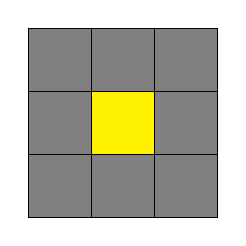
\begin{tikzpicture}[scale=0.8]
    % Draw the 3x3 Top Face Grid
    \foreach \x in {0,1,2} {
        \foreach \y in {0,1,2} {
            \draw[fill=gray] (\x,\y) rectangle (\x+1,\y+1);
        }
    }

    \foreach \x/\y in {1/1} {
        \draw[fill=yellow] (\x,\y) rectangle (\x+1,\y+1);
    }
\end{tikzpicture}

\medskip
\texttt{f (R U R' U') f' U \\ F (R U R' U') F'}

\centering
\subsubsection*{Line case}
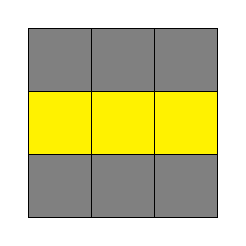
\begin{tikzpicture}[scale=0.8]
    % Draw the 3x3 Top Face Grid
    \foreach \x in {0,1,2} {
        \foreach \y in {0,1,2} {
            \draw[fill=gray] (\x,\y) rectangle (\x+1,\y+1);
        }
    }

    \foreach \x/\y in {0/1, 1/1, 2/1} {
        \draw[fill=yellow] (\x,\y) rectangle (\x+1,\y+1);
    }
\end{tikzpicture}

\medskip
\texttt{F (R U R' U') F'}

\centering
\subsubsection*{Anti-Sune}
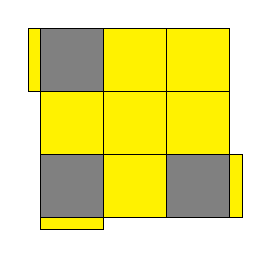
\begin{tikzpicture}[scale=0.8]
    % Draw the 3x3 Top Face Grid
    \foreach \x in {0,1,2} {
        \foreach \y in {0,1,2} {
            \draw[fill=gray] (\x,\y) rectangle (\x+1,\y+1);
        }
    }

    \foreach \x/\y in {0/1, 1/0, 1/1, 1/2, 2/1, 2/2} {
        \draw[fill=yellow] (\x,\y) rectangle (\x+1,\y+1);
    }

    \draw[fill=yellow] (0,-0.2) rectangle (1,0);
    \draw[fill=yellow] (3,0) rectangle (3.2,1);
    \draw[fill=yellow] (-0.2,2) rectangle (0,3);
\end{tikzpicture}

\medskip
\texttt{R U2 R' U' R U' R'}

\centering
\subsubsection*{Cross 2}
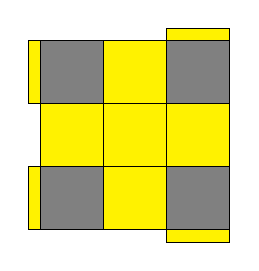
\begin{tikzpicture}[scale=0.8]
    % Draw the 3x3 Top Face Grid
    \foreach \x in {0,1,2} {
        \foreach \y in {0,1,2} {
            \draw[fill=gray] (\x,\y) rectangle (\x+1,\y+1);
        }
    }

    \foreach \x/\y in {0/1, 1/0, 1/1, 1/2, 2/1} {
        \draw[fill=yellow] (\x,\y) rectangle (\x+1,\y+1);
    }

    \draw[fill=yellow] (-0.2,0) rectangle (0,1);
    \draw[fill=yellow] (2,-0.2) rectangle (3,0);
    \draw[fill=yellow] (-0.2,2) rectangle (0,3);
    \draw[fill=yellow] (2,3.2) rectangle (3,3);
\end{tikzpicture}

\medskip
\texttt{R U2 R2 U' R2 U' R2 U2 R}

\centering
\subsubsection*{Kite}
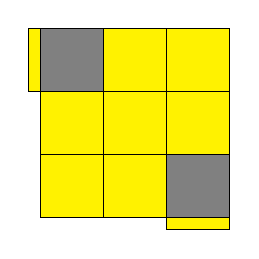
\begin{tikzpicture}[scale=0.8]
    % Draw the 3x3 Top Face Grid
    \foreach \x in {0,1,2} {
        \foreach \y in {0,1,2} {
            \draw[fill=gray] (\x,\y) rectangle (\x+1,\y+1);
        }
    }

    \foreach \x/\y in {0/0, 0/1, 1/0, 1/1, 1/2, 2/1, 2/2} {
        \draw[fill=yellow] (\x,\y) rectangle (\x+1,\y+1);
    }

    \draw[fill=yellow] (2,-0.2) rectangle (3,0);
    \draw[fill=yellow] (-0.2,2) rectangle (0,3);
\end{tikzpicture}

\medskip
\texttt{F' r U R' U' r' F R}
\end{minipage}%
\hfill
\begin{minipage}{0.45\textwidth}
\centering
\subsubsection*{L case}
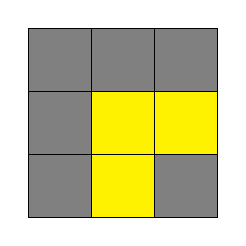
\begin{tikzpicture}[scale=0.8]
    % Draw the 3x3 Top Face Grid
    \foreach \x in {0,1,2} {
        \foreach \y in {0,1,2} {
            \draw[fill=gray] (\x,\y) rectangle (\x+1,\y+1);
        }
    }

    \foreach \x/\y in {1/0, 1/1, 2/1} {
        \draw[fill=yellow] (\x,\y) rectangle (\x+1,\y+1);
    }
\end{tikzpicture}

\medskip
\texttt{f (R U R' U') f'}

\centering
\subsubsection*{Sune}
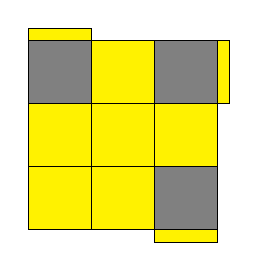
\begin{tikzpicture}[scale=0.8]
    % Draw the 3x3 Top Face Grid
    \foreach \x in {0,1,2} {
        \foreach \y in {0,1,2} {
            \draw[fill=gray] (\x,\y) rectangle (\x+1,\y+1);
        }
    }

    \foreach \x/\y in {0/0, 0/1, 1/0, 1/1, 1/2, 2/1} {
        \draw[fill=yellow] (\x,\y) rectangle (\x+1,\y+1);
    }

    \draw[fill=yellow] (2,0) rectangle (3,-0.2);
    \draw[fill=yellow] (3,2) rectangle (3.2,3);
    \draw[fill=yellow] (0,3) rectangle (1,3.2);
\end{tikzpicture}

\medskip
\texttt{R U R' U R U2 R'}

\centering
\subsubsection*{Cross 1}
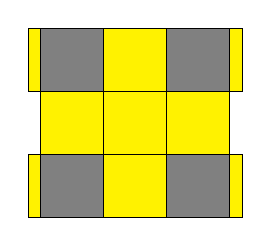
\begin{tikzpicture}[scale=0.8]
    % Draw the 3x3 Top Face Grid
    \foreach \x in {0,1,2} {
        \foreach \y in {0,1,2} {
            \draw[fill=gray] (\x,\y) rectangle (\x+1,\y+1);
        }
    }

    \foreach \x/\y in {0/1, 1/0, 1/1, 1/2, 2/1} {
        \draw[fill=yellow] (\x,\y) rectangle (\x+1,\y+1);
    }

    \draw[fill=yellow] (-0.2,0) rectangle (0,1);
    \draw[fill=yellow] (-0.2,2) rectangle (0,3);
    \draw[fill=yellow] (3,0) rectangle (3.2,1);
    \draw[fill=yellow] (3,2) rectangle (3.2,3);
\end{tikzpicture}

\medskip
\texttt{R U R' U R U' R' U R U2 R'}

\centering
\subsubsection*{Chameleon}
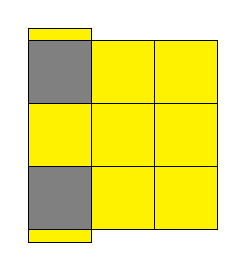
\begin{tikzpicture}[scale=0.8]
    % Draw the 3x3 Top Face Grid
    \foreach \x in {0,1,2} {
        \foreach \y in {0,1,2} {
            \draw[fill=gray] (\x,\y) rectangle (\x+1,\y+1);
        }
    }

    \foreach \x/\y in {0/1, 1/0, 1/1, 1/2, 2/0, 2/1, 2/2} {
        \draw[fill=yellow] (\x,\y) rectangle (\x+1,\y+1);
    }

    \draw[fill=yellow] (0,-0.2) rectangle (1,0);
    \draw[fill=yellow] (0,3.2) rectangle (1,3);
\end{tikzpicture}

\medskip
\texttt{r U R' U' r' F R F'}

\centering
\subsubsection*{Headlights}
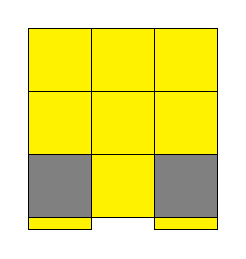
\begin{tikzpicture}[scale=0.8]
    % Draw the 3x3 Top Face Grid
    \foreach \x in {0,1,2} {
        \foreach \y in {0,1,2} {
            \draw[fill=gray] (\x,\y) rectangle (\x+1,\y+1);
        }
    }

    \foreach \x/\y in {0/1, 0/2, 1/0, 1/1, 1/2, 2/1, 2/2} {
        \draw[fill=yellow] (\x,\y) rectangle (\x+1,\y+1);
    }

    \draw[fill=yellow] (0,-0.2) rectangle (1,0);
    \draw[fill=yellow] (2,-0.2) rectangle (3,0);
\end{tikzpicture}

\medskip
\texttt{R2 D R' U2 R D' R' U2 R'}
\end{minipage}
\newpage
\section*{2-look PLL Algorithms}

% --- OLL CASE (e.g., OLL 21 / Cross "Cross") ---
\begin{minipage}{0.45\textwidth}
\centering
\subsubsection*{Y-perm}
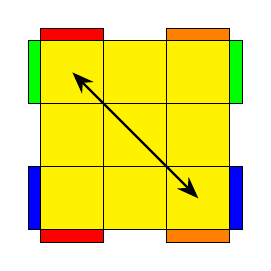
\begin{tikzpicture}[scale=0.8]
    % Draw the 3x3 Top Face Grid
    \foreach \x in {0,1,2} {
        \foreach \y in {0,1,2} {
            \draw[fill=yellow] (\x,\y) rectangle (\x+1,\y+1);
        }
    }
    % Color the oriented yellow stickers on top
    % Add OLL unoriented bars on the side (thick outer lines)
    % Example: Yellow facing outward on the bottom layer sides
    \draw[fill=red] (0,0) rectangle (1,-0.2);
    \draw[fill=blue] (0,0) rectangle (-0.2,1);
    
    \draw[fill=orange] (2,0) rectangle (3,-0.2);
    \draw[fill=blue] (3,0) rectangle (3.2,1);

    \draw[fill=green] (3,2) rectangle (3.2,3);
    \draw[fill=orange] (2,3.2) rectangle (3,3);

    \draw[fill=green] (-0.2,2) rectangle (0,3);
    \draw[fill=red] (0,3.2) rectangle (1,3);
    % \draw[line width=3pt, red] (0,-0.1) -- (1,-0.1);
    % \draw[line width=3pt, yellow] (2,0) -- (2,1);
    % \draw[line width=3pt, yellow] (3,1) -- (3,2);

    \draw[pllarrow2] (0.5, 2.5) to[bend right=0] (2.5, 0.5);
\end{tikzpicture}

\medskip
\texttt{F R U' R' U' R U R' F' \\ (R U R' U') R' F R F'}

\centering
\subsubsection*{Ua-Perm}
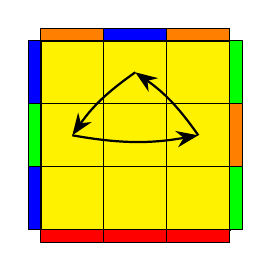
\begin{tikzpicture}[scale=0.8]
    % Draw a completely solved top yellow face
    \foreach \x in {0,1,2} {
        \foreach \y in {0,1,2} {
            \draw[fill=yellow] (\x,\y) rectangle (\x+1,\y+1);
        }
    }
    % Outer boundary of the cube top view
    \draw[thick] (0,0) rectangle (3,3);

    \draw[fill=red] (0,0) rectangle (1,-0.2);
    \draw[fill=blue] (0,0) rectangle (-0.2,1);
    
    \draw[fill=red] (2,0) rectangle (3,-0.2);
    \draw[fill=green] (3,0) rectangle (3.2,1);

    \draw[fill=green] (3,2) rectangle (3.2,3);
    \draw[fill=orange] (2,3.2) rectangle (3,3);

    \draw[fill=blue] (-0.2,2) rectangle (0,3);
    \draw[fill=orange] (0,3.2) rectangle (1,3);

    %edges
    \draw[fill=red] (1,0) rectangle (2,-0.2);
    
    \draw[fill=orange] (3,1) rectangle (3.2,2);

    \draw[fill=blue] (1,3.2) rectangle (2,3);

    \draw[fill=green] (-0.2,2) rectangle (0,1);
    
    % Draw Permutation Arrows (using centers of the 3x3 grid cells)
    % Ua perm cycles edges: Front -> Right -> Left
    \draw[pllarrow] (2.5, 1.5) to[bend right=10] (1.5, 2.5); % F edge to R edge
    \draw[pllarrow] (0.5, 1.5) to[bend right=10] (2.5, 1.5); % R edge to L edge
    \draw[pllarrow] (1.5, 2.5) to[bend right=10] (0.5, 1.5); % L edge to F edge
\end{tikzpicture}

\medskip
\texttt{R2 U' R' U' R U R U R U' R}

\centering
\subsubsection*{H-Perm}
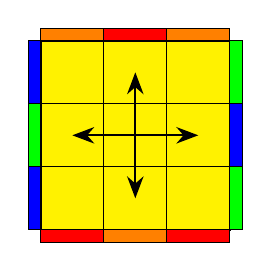
\begin{tikzpicture}[scale=0.8]
    % Draw a completely solved top yellow face
    \foreach \x in {0,1,2} {
        \foreach \y in {0,1,2} {
            \draw[fill=yellow] (\x,\y) rectangle (\x+1,\y+1);
        }
    }
    % Outer boundary of the cube top view
    \draw[thick] (0,0) rectangle (3,3);

    \draw[fill=red] (0,0) rectangle (1,-0.2);
    \draw[fill=blue] (0,0) rectangle (-0.2,1);
    
    \draw[fill=red] (2,0) rectangle (3,-0.2);
    \draw[fill=green] (3,0) rectangle (3.2,1);

    \draw[fill=green] (3,2) rectangle (3.2,3);
    \draw[fill=orange] (2,3.2) rectangle (3,3);

    \draw[fill=blue] (-0.2,2) rectangle (0,3);
    \draw[fill=orange] (0,3.2) rectangle (1,3);
    
    %edges
    \draw[fill=orange] (1,0) rectangle (2,-0.2);
    
    \draw[fill=blue] (3,1) rectangle (3.2,2);

    \draw[fill=red] (1,3.2) rectangle (2,3);

    \draw[fill=green] (-0.2,2) rectangle (0,1);
    
    % Draw Permutation Arrows (using centers of the 3x3 grid cells)
    % Ub perm cycles edges: Front -> Right -> Left
    \draw[pllarrow2] (1.5, 2.5) to[bend left=0] (1.5, 0.5); % F edge to R edge
    \draw[pllarrow2] (2.5, 1.5) to[bend left=0] (0.5, 1.5); % R edge to L edge
\end{tikzpicture}

\medskip
\texttt{M2 U' M2 U2 M2 U' M2}
\end{minipage}%
\hfill
% --- PLL CASE (e.g., U-Permutation) ---
\begin{minipage}{0.45\textwidth}
\centering
\subsubsection*{T-perm}
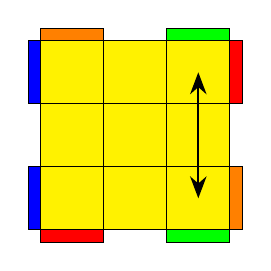
\begin{tikzpicture}[scale=0.8]
    % Draw the 3x3 Top Face Grid
    \foreach \x in {0,1,2} {
        \foreach \y in {0,1,2} {
            \draw[fill=yellow] (\x,\y) rectangle (\x+1,\y+1);
        }
    }
    % Add OLL unoriented bars on the side (thick outer lines)
    % Example: Yellow facing outward on the bottom layer sides
    \draw[fill=red] (0,0) rectangle (1,-0.2);
    \draw[fill=blue] (0,0) rectangle (-0.2,1);
    
    \draw[fill=green] (2,0) rectangle (3,-0.2);
    \draw[fill=orange] (3,0) rectangle (3.2,1);

    \draw[fill=red] (3,2) rectangle (3.2,3);
    \draw[fill=green] (2,3.2) rectangle (3,3);

    \draw[fill=blue] (-0.2,2) rectangle (0,3);
    \draw[fill=orange] (0,3.2) rectangle (1,3);
    % \draw[line width=3pt, yellow] (0,0) -- (0,1);
    % \draw[line width=3pt, yellow] (2,0) -- (2,1);
    % \draw[line width=3pt, yellow] (3,1) -- (3,2);
    \draw[pllarrow2] (2.5, 2.5) to[bend right=0] (2.5, 0.5);
\end{tikzpicture}

\medskip
\texttt{(R U R' U') R' F R2 \\ U' R' U' R U R' F'}

\centering
\subsubsection*{Ub-Perm}
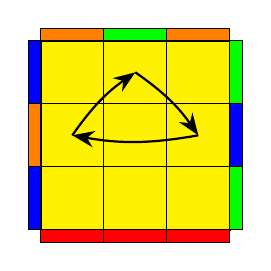
\begin{tikzpicture}[scale=0.8]
    % Draw a completely solved top yellow face
    \foreach \x in {0,1,2} {
        \foreach \y in {0,1,2} {
            \draw[fill=yellow] (\x,\y) rectangle (\x+1,\y+1);
        }
    }
    % Outer boundary of the cube top view
    \draw[thick] (0,0) rectangle (3,3);

    \draw[fill=red] (0,0) rectangle (1,-0.2);
    \draw[fill=blue] (0,0) rectangle (-0.2,1);
    
    \draw[fill=red] (2,0) rectangle (3,-0.2);
    \draw[fill=green] (3,0) rectangle (3.2,1);

    \draw[fill=green] (3,2) rectangle (3.2,3);
    \draw[fill=orange] (2,3.2) rectangle (3,3);

    \draw[fill=blue] (-0.2,2) rectangle (0,3);
    \draw[fill=orange] (0,3.2) rectangle (1,3);
    
    %edges
    \draw[fill=red] (1,0) rectangle (2,-0.2);
    
    \draw[fill=blue] (3,1) rectangle (3.2,2);

    \draw[fill=green] (1,3.2) rectangle (2,3);

    \draw[fill=orange] (-0.2,2) rectangle (0,1);
    
    % Draw Permutation Arrows (using centers of the 3x3 grid cells)
    % Ub perm cycles edges: Front -> Right -> Left
    \draw[pllarrow] (1.5, 2.5) to[bend left=10] (2.5, 1.5); % F edge to R edge
    \draw[pllarrow] (2.5, 1.5) to[bend left=10] (0.5, 1.5); % R edge to L edge
    \draw[pllarrow] (0.5, 1.5) to[bend left=10] (1.5, 2.5); % L edge to F edge
\end{tikzpicture}

\medskip
\texttt{R' U R' U' R' U' R' U R U R2}

\centering
\subsubsection*{Z-Perm}
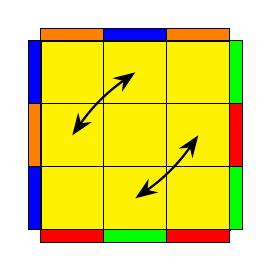
\begin{tikzpicture}[scale=0.8]
    % Draw a completely solved top yellow face
    \foreach \x in {0,1,2} {
        \foreach \y in {0,1,2} {
            \draw[fill=yellow] (\x,\y) rectangle (\x+1,\y+1);
        }
    }
    % Outer boundary of the cube top view
    \draw[thick] (0,0) rectangle (3,3);

    \draw[fill=red] (0,0) rectangle (1,-0.2);
    \draw[fill=blue] (0,0) rectangle (-0.2,1);
    
    \draw[fill=red] (2,0) rectangle (3,-0.2);
    \draw[fill=green] (3,0) rectangle (3.2,1);

    \draw[fill=green] (3,2) rectangle (3.2,3);
    \draw[fill=orange] (2,3.2) rectangle (3,3);

    \draw[fill=blue] (-0.2,2) rectangle (0,3);
    \draw[fill=orange] (0,3.2) rectangle (1,3);
    
    %edges
    \draw[fill=green] (1,0) rectangle (2,-0.2);
    
    \draw[fill=red] (3,1) rectangle (3.2,2);

    \draw[fill=blue] (1,3.2) rectangle (2,3);

    \draw[fill=orange] (-0.2,2) rectangle (0,1);
    
    % Draw Permutation Arrows (using centers of the 3x3 grid cells)
    % Ub perm cycles edges: Front -> Right -> Left
    \draw[pllarrow2] (2.5, 1.5) to[bend left=10] (1.5, 0.5); % F edge to R edge
    \draw[pllarrow2] (0.5, 1.5) to[bend left=10] (1.5, 2.5); % R edge to L edge
\end{tikzpicture}

\medskip
\texttt{M' U' M2 U' M2 U' M' U2 M2}
\end{minipage}

\end{document}